%!TEX root = practicum1.tex
We perform two different experiments with the Chirikov map defined in \cref{eq:chirikov}. In \cref{ss:fixed} we fix the value of the non-linearity parameter and explore the influences of different values for $p_0$ and $x_0$. In \cref{ss:variable} we discuss the influence of the non-linearity parameter $K$. Plotting various Chirikov maps with randomly chosen initial conditions for $K = 1$ results in decorative images, such as the one presented in \cref{fig:a:pretty}.

	\begin{figure}[b]
		\centering
		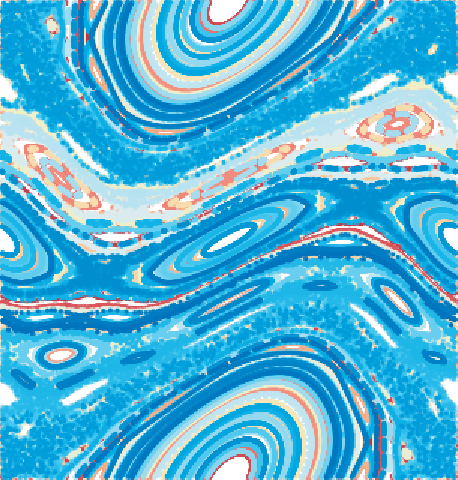
\includegraphics[width=0.9\columnwidth]{./img/assignment_a_pretty_low_res.pdf}
		\caption{500 randomly initialized orbits of the Frenkel-Kontorova model for $K = 1$.}
		\label{fig:a:pretty}
	\end{figure}

\subsection[]{Fixed $K$}
\label{ss:fixed}
	We have fixed the value of $K$ to 1, essentially removing the parameter from the equation. By choosing different initial values we can generate discrete points, close curves and orbits with \cref{eq:chirikov}.
	
	\subsubsection{Discrete points}
	We have generated a one-dimensional Chirikov map by choosing $x_0 = p_0 = 0.5$. Using these values $p_1 = p_0$ since the second term of \eqref{eq:chirikov:p} becomes zero. This results in $x_1 = \left( x_0 + p_{1} \right) \mod 1= 0$. The next steps are easily derived since $p_{n + 1}$ for $n > 0$ will not change due to the fact that both 0 and 0.5 as input to \eqref{eq:chirikov:p} will result in the second term becoming zero. With this initialization $x_{n} \in \left\{0,\, 0.5 \right\} \text{ for } n \geq 0$. To illustrate $x_2$ is $0.5 + 0 = 0.5$ which is equal to $x_1$. We have now shown that $p_n$ is constant for $n \geq 1$ and that $x_n$ jumps between 0 and 0.5, which explains the results in \cref{fig:experiment:dimension:0}. 

	Furthermore we have shown that these points are visited in a fixed order, which explains the plots in \crefrange{fig:experiment:dimension:0:x}{fig:experiment:dimension:0:p}.\\

	From this specific case we can derive the following constraints for $p_0$ and $x_0$; $x_0$ should be chosen in such a way that the sine in \cref{eq:chirikov:p} becomes 0, i.e. $x_0 \in \{0,\, 0.5,\, 1\}$. Due to the constraint on $x_0$,
	\begin{equation*}
	p_{n + 1} = p_{n} \mod 1,
	\end{equation*}
 	which is equal to $p_n$, unless $p_n = 1$. Consquently
 	\begin{equation}
 	x_{n + 1} = x_n + p_n \mod 1,
 	\end{equation}
	unless $p_1 = 1$. Formally, one should choose $p_0$ in such a way that:
	\begin{equation*}
		\left( \left[ x_0 + (p_0 \mod 1)\right] \mod 1 \right) \in \left\{0, 0.5, 1\right\}.
	\end{equation*}

	\subsubsection{Closed curves}
	We have determined empircally that $\left\{x_0\,, p_0 \right\} = {\num{0.1269868},\,\num{0.9133759}}$ results in closed curves. \Cref{fig:experiment:dimension:1} shows $p_n$ as a function of $x_n$, \crefrange{fig:experiment:dimension:1:x}{fig:experiment:dimension:1:p} shows the progression of respectively $p$ and $x$. 

	\todo[inline]{Are the single points or curves visited in a fixed order?}
	\todo[inline]{What happens in the filled areas?}

	\subsubsection{Orbits}	
	\todo[inline]{Wanneer krijgen we dit?}
	\todo[inline]{Are the single points or curves visited in a fixed order?}
	\todo[inline]{What happens in the filled areas?}

	%!TEX root = practicum1.tex

\begin{figure*}
	\centering
	% \x/\picname in {4/pic1.png,8/pic2.png,15/pic3.png,16/pic4.png}
	\foreach \dim/\x/\p in {0/0.500/0.500, 1/0.1576131/0.9705928, 2/0.1269868/0.9133759}
	{ 
		\begin{subfigure}[t]{0.32\textwidth}
			\includegraphics[width=\textwidth]{./img/assignment_a_\dim_dim.pdf}
			\caption{$x_0=\num{\x}$, $p_0=\num{\p}$}
			\label{fig:experiment:dimension:\dim}
		\end{subfigure}
		\begin{subfigure}[t]{0.32\textwidth}
			\includegraphics[width=\textwidth]{./img/assignment_a_\dim_dim_progression_p.pdf}
			\caption{Progression of $p$ in \subref{fig:experiment:dimension:\dim}}
			\label{fig:experiment:dimension:\dim:x}
		\end{subfigure}		
		\begin{subfigure}[t]{0.32\textwidth}
			\includegraphics[width=\textwidth]{./img/assignment_a_\dim_dim_progression_x.pdf}
			\caption{Progression of $x$ in \subref{fig:experiment:dimension:\dim}}
			\label{fig:experiment:dimension:\dim:p}
		\end{subfigure}		
	}
	\caption{Each row corresponds to on set of initial values $\left\langle x_0, p_0 \right\rangle$. The first column shows $x_n$ versus $p_n$ for $n \in \left[0,\, \num{10000} \right]$. The second and third column depict respectively the progression of $p$ and $x$.}
	\label{fig:experiment:dimension}
\end{figure*}

\subsection[]{Variable $K$}
\label{ss:variable}